\documentclass{beamer}
\usepackage{beamerthemesplit}
\usepackage{wrapfig}
\usetheme{SPbGU}
\usepackage{pdfpages}
\usepackage{amsmath}
\usepackage{cmap} 
\usepackage[T2A]{fontenc} 
\usepackage[utf8]{inputenc}
\usepackage[english,russian]{babel}
\usepackage{indentfirst}
\usepackage{amsmath}
\usepackage{tikz}
\usepackage{multirow}
\usepackage[noend]{algpseudocode}
\usepackage{algorithm}
\usepackage{algorithmicx}
\usetikzlibrary{shapes,arrows}
\usepackage{fancyvrb}
\newtheorem{rutheorem}{Теорема}
\newtheorem{ruproof}{Доказательство}
\newtheorem{rudefinition}{Определение}
\newtheorem{rulemma}{Лемма}
\beamertemplatenavigationsymbolsempty
\usepackage{pgfplots}
\pgfplotsset{compat=1.9}


\title[]{\large Реализация алгоритма поиска минимального остовного дерева с использованием библиотеки SuiteSparse}
\subtitle[]{} 
\institute[СПбГУ]{
Санкт-Петербургский государственный университет \\
Кафедра системного программирования }
\author[Суханова Анжела]{Суханова Анжела Кирилловна, 271 группа (18.Б11-мм) \\
  \and  
     {\bfseries Научный руководитель:} доцент кафедры информатики СПбГУ, к.ф.-м.н. Григорьев С.\,В.}

\date{6 июня 2020г.}

\definecolor{orange}{RGB}{179,36,31}

\begin{document}
{
% Лого университета или организации, отображается в шапке титульного листа
\begin{frame}
  \begin{center}
  {
\includegraphics[width=1.5cm]{pictures/SPbGU_Logo.png}}
  \end{center}
  \titlepage
\end{frame}
}

\begin{frame}[fragile]
  \transwipe[direction=90]
  \frametitle{Введение}
  \begin{itemize}
    \item Анализ графструктурированных данных находит применение в биоинформатике, анализе социальных сетей, молекулярном синтезе, планировании маршрутов
    \item Высокопроизводительные реализации графовых алгоритмов сложно представлять на новом параллельном оборудовании
    \item GraphBLAS~--- открытый стандарт, определяющий структурные блоки графовых алгоритмов на языке линейной алгебры
    \item SuiteSparse: GraphBLAS~--- первая полная реализация стандарта GraphBLAS
    \item Aлгоритм поиска минимального остовного деревa (MST) применяется в различных практических и теоретических областях
  \end{itemize}
\end{frame}
            

% Обязательный слайд: четкая формулировка цели данной работы и постановка задачи
% Описание выносимых на защиту результатов, процесса или особенностей их достижения и т.д.
\begin{frame}
  \transwipe[direction=90]
  \frametitle{Постановка задачи}
  \textbf{Целью} данной работы является реализация алгоритма поиска минимального остовного дерева 
на SuiteSparse: GraphBLAS

  \textbf{Задачи}:
  \begin{itemize}
    \item Собрать и изучить SuiteSparse
    \item Реализовать алгоритм поиска минимального остовного дерева на SuiteSparse
    \item Провести экспериментальное исследование реализации
  \end{itemize}
\end{frame}


\begin{frame}
  \transwipe[direction=90]
  \frametitle{Алгоритм Борувки}
  \begin{itemize}
	\item Изначально каждая вершина графа~--- тривиальное дерево, а ребра не принадлежат никакому дереву
	\item Для каждого дерева находится минимальное инцидентное ему ребро, все такие рёбра добавляются к деревьям
	\item Второй шаг повторяется, пока в графе не останется только одно дерево
  \end{itemize}
  \begin{figure}[h]
      \center{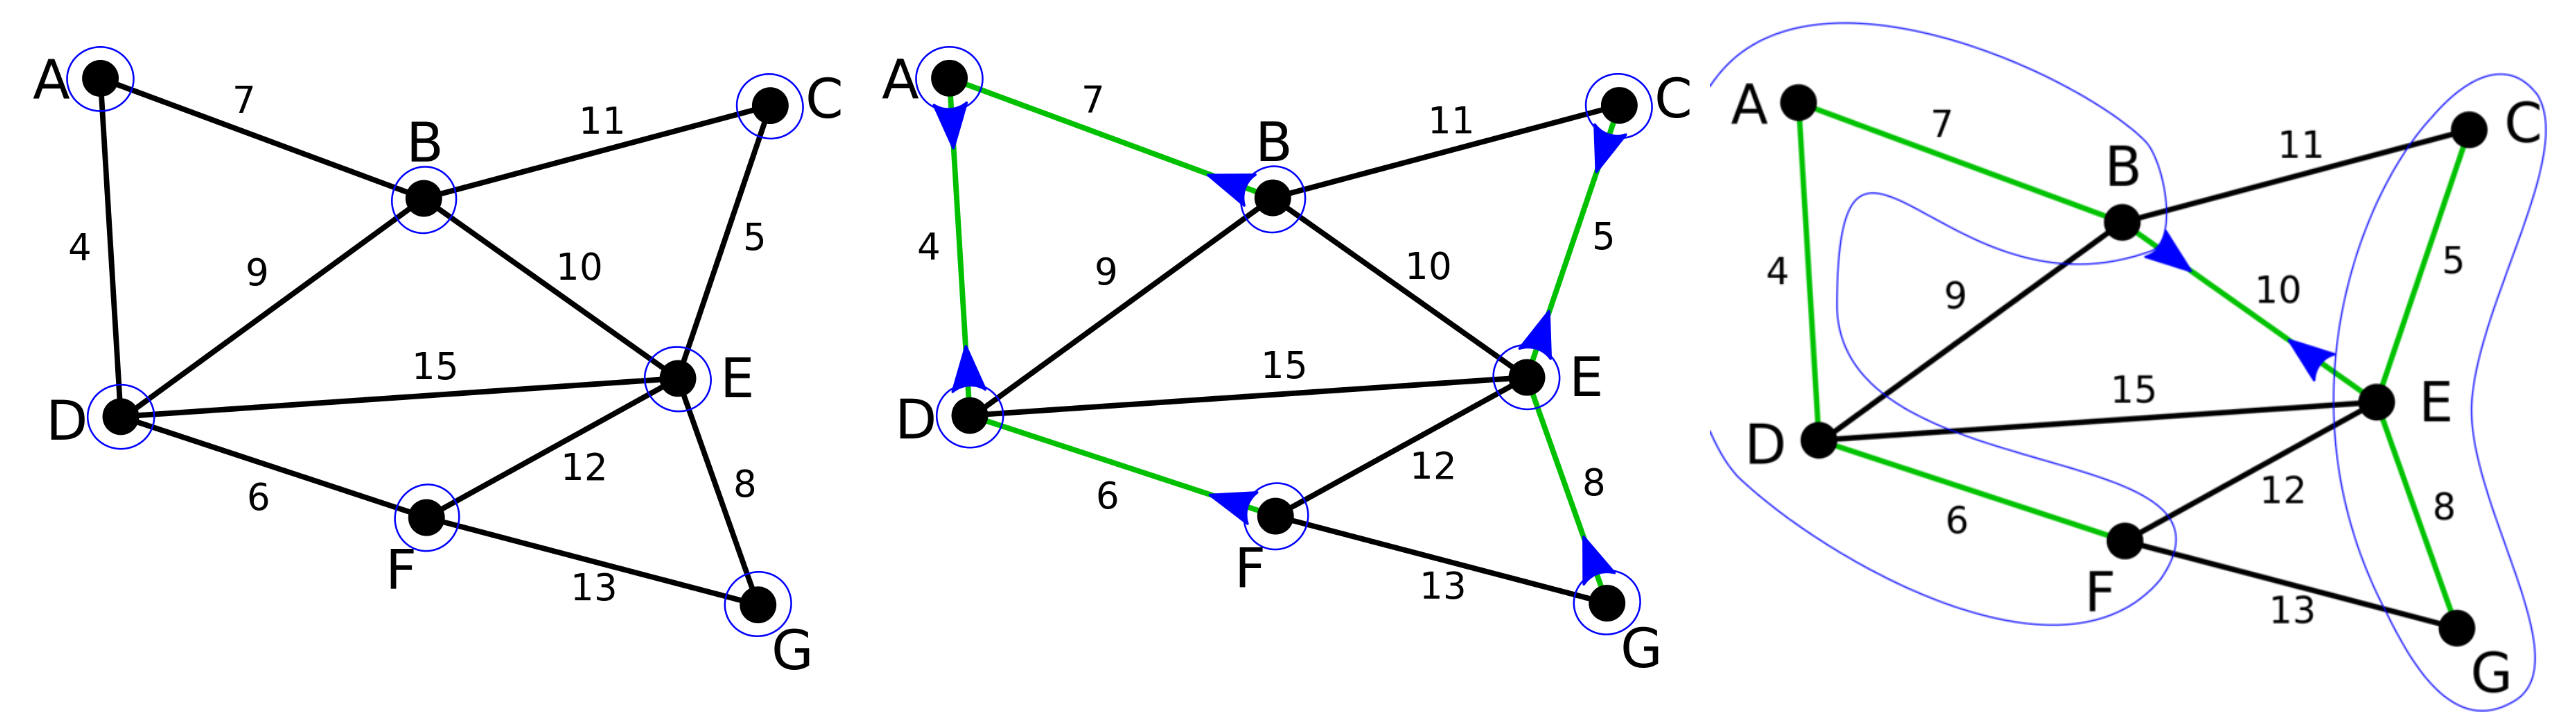
\includegraphics[scale=0.135]{pictures/Boruvka}}
      \begin{flushright}
          \textcolor{darkgray}{\tiny Схема взята из \url{https://en.wikipedia.org/wiki/Bor\%C5\%AFvka\%27s\_algorithm}}
      \end{flushright}
  \end{figure}
\end{frame}


\begin{frame}
  \transwipe[direction=90]
  \frametitle{Архитектура решения}
	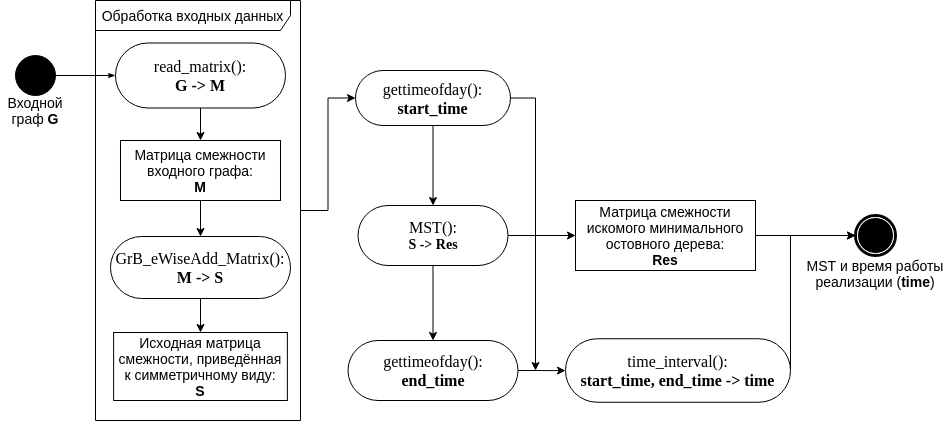
\includegraphics[width=\textwidth]{pictures/Diagram}
\end{frame}


\begin{frame}
  \transwipe[direction=90]
  \frametitle{\large Экспериментальное исследование на плотных графах}
  \begin{tikzpicture}[scale=.77]
  \begin{semilogyaxis}[
    xlabel = {№ теста},
    ylabel = {Среднее время работы реализаций, сек},
    legend pos={south east}
  ]
  \addplot[
    mark size=2pt,
    only marks,
    point meta=explicit symbolic,
    scatter,
    scatter/classes={
		a={red}, 
		b={blue}, 
		c={green} 
	}]
  table [meta=class, row sep=crcr]{
	x  y  class   \\
	1  0.000766  a \\
	1  0.000176  b \\
	1  0.000820  c \\
	2  0.130250  a \\
	2  19.642873  b \\
	2  0.077085  c \\
	3  1.447504  a \\
	3  2270.556707  b \\
	3  1.350120  c \\
	4  1.797109  a \\
	4  13090.249882  b \\
        4  3.800798  c \\
        5  3.575253  a \\
        5  5.245117  c \\
        6  5.733534  a \\
        6  8.056583  c \\
  };
  \legend{SuiteSparse, GBTL, LAGraph}
  \end{semilogyaxis}
  \end{tikzpicture}
  \begin{table}[ht]
  \centering
  \scalebox{0.63}[0.63]{
	\begin{tabular}{|c|c|c|c|c|c|c|}\hline
		 № теста & Число рёбер & Число вершин & Диапaзон весов & SuiteSparse (сек) & GBTL (сек) & LAGraph (сек) \\\hline
                 1 & 8 & 4 & 1 & 0.0008 & 0.0002 & 0.0008 \\\hline
		 2 & 499500 & 1000 & [1, 5000] & 0.1303 & 19.6429 & 0.0771 \\\hline
		 3 & 12497500 & 5000 & [1, 5000] & 1.4475 & 2270.5567 & 1.3501 \\\hline
		 4 & 40495500 & 9000 & [1, 1000] & 1.7971 & 13090.2499 & 3.8008 \\\hline
                 5 & 40495500 & 9000 & [1, $10^4$] & 3.5753 && 5.2451 \\\hline
                 6 & 49995000 & $10^4$ & [1, $10^5$] & 5.7335 && 8.0566 \\\hline
	\end{tabular}
  }
  \end{table}
\end{frame}


\begin{frame}
  \transwipe[direction=90]
  \frametitle{\large Экспериментальное исследование на разрежённых графах}
  \begin{tikzpicture}[scale=.77]
  \begin{semilogyaxis}[
    xlabel = {№ теста},
    ylabel = {Среднее время работы реализаций, сек},
    legend pos={north west}
  ]
  \addplot[
    mark size=2pt,
    only marks,
    point meta=explicit symbolic,
    scatter,
    scatter/classes={
		a={red}, 
		b={blue}, 
		c={green}}]
  table [meta=class, row sep=crcr]{
	x  y  class \\
	1  0.001292  a \\
	1  0.000776  b \\
	1  0.000868  c \\
	2  0.005713  a \\
	2  0.039466  b \\
	2  0.001101  c \\
	3  1.066108  a \\
	3  131.830707  b \\
	3  0.022403  c \\
	4  1.064990  a \\
	4  132.101915  b \\
        4  0.023217  c \\
        5  1.085588  a \\
	5  160.264775  b \\
        5  0.022630  c \\
        6  160.169242  a \\
        6  2.285694  c \\
  };
  \legend{SuiteSparse, GBTL, LAGraph}
  \end{semilogyaxis}
  \end{tikzpicture}
  \begin{table}[ht]
  \centering
  \scalebox{0.63}[0.63]{
	\begin{tabular}{|c|c|c|c|c|c|c|}\hline
		 № теста & Число рёбер & Число вершин & Диапaзон весов & SuiteSparse (сек) & GBTL (сек) & LAGraph (сек) \\\hline
                 1 & 16 & 10 & 1 & 0.0013 & 0.0008 & 0.0009 \\\hline
		 2 & 196 & 100 & 1 & 0.0057 & 0.0395 & 0.0011 \\\hline
                 3 & 19996 & $10^4$ & [1, 1000] & 1.0661 & 131.8307 & 0.0224 \\\hline
		 4 & 19996 & $10^4$ & [1, $10^4$] & 1.0650 & 132.1019 & 0.0232 \\\hline
		 5 & 99900 & $10^4$ & [1, $10^4$] & 1.0856 & 160.2648 & 0.0226 \\\hline
		 6 & 9999900 & $10^6$ & [1, $10^6$] & 160.1692 && 2.2857 \\\hline
	\end{tabular}
  }
  \end{table}
\end{frame}


\begin{frame}
  \transwipe[direction=90]
  \frametitle{Результаты}
  \begin{itemize}
    \item Осуществлены сборка и изучение библиотеки высокопроизводительной обработки графов SuiteSparse
    \item Реализован алгоритм поиска MST на SuiteSparse: GraphBLAS
    \item Проведено исследование производительности реализации, в том числе сравнение с представлениями алгоритмов поиска MST на других библиотеках, основанных на GraphBLAS
  \end{itemize}
\end{frame}

\end{document}
